\section{Methods}
\label{sec:methods}

\subsection{Model System}

Experiments testing the relationships between evolutionary dynamics, reconstruction error, and phylogenetic structure required a model system amenable to direct, interpretable tuning of ecology, spatial structure, and selection pressure.
Additionally, in order to make findings relevant to large-scale phylogenetic analyses, computational efficiency was necessary to facilitate large population size and high generation counts.
Finally, a parsimonious and generic model system was desired so that findings would better generalize across digital evolution systems.

A parsimonious model system was devised to fulfill these objectives.
Genomes in this system comprised a single floating-point value, with higher magnitude corresponding to higher fitness.
Population size 32,768 ($2^{15}$) was used for all experiments.
Selection was performed using tournament selection with synchronous generations.
Treatments' selection pressure was controlled via tournament size.
Mutation was applied after selection, with a value drawn from a unit Gaussian distribution added to all genomes.
Evolutionary runs were ended after 262,144 ($2^{18}$) generations.
Each run required around 4 hours of compute time.

Treatments incorporating spatial structure used a simple island model.
In spatially structured treatments, individuals were evenly divided among 1,024 islands and only competed in selection tournaments against sympatric population members.
Islands were arranged in a one-dimensional closed ring and 1\% of population members migrated to a neighboring island each generation.

Treatments incorporating ecology used a simple niche model.
Population slots were split evenly between niches.
Organisms were arbitrarily assigned to a niche at genesis and were only allowed to occupy population slots assigned to that niche.
Therefore, individuals exclusively participated in selection tournaments with members of their own niche.
In treatments also incorporating spatial structure, an even allotment of population slots was provided for every niche on every island.
Every generation, individuals swapped niches with probability $3.0517578125 \times 10^{-8}$ (chosen so one niche swap would be expected every 1,000 generations).

For our main experiments, we defined the following ``regimes'' of evolutionary conditions:
\begin{itemize}
  \item \textit{plain}: tournament size 2 with no niching and no islands,
  \item \textit{weak selection}: tournament size 1 with no niching and no islands,
  \item \textit{strong selection}: tournament size 4 with no niching and no islands,
  \item \textit{spatial structure}: tournament size 2 with no niching and 1,024 islands,
  \item \textit{weak 4 niche ecology}: tournament size 2 with 4 niches and niche swap probability increased 100$\times$,
  \item \textit{4 niche ecology}: tournament size 2 with 4 niches, and
  \item \textit{8 niche ecology}: tournament size 8 with 4 niches.
\end{itemize}

In follow-up experiments testing ecological dynamics with a spatial background, we defined the following additional evolutionary ``regimes:''
\begin{itemize}
  \item \textit{plain}: tournament size 2 with no niching over 1,024 islands,
  \item \textit{weak 4 niche ecology}: tournament size 2 with 4 niches and niche swap probability increased 100$\times$ over 1,024 islands,
  \item \textit{4 niche ecology}: tournament size 2 with 4 niches over 1,024 islands, and
  \item \textit{8 niche ecology}: tournament size 8 with 4 niches over 1,024 islands.
\end{itemize}

Finally, to foster generalizability of findings, all experiments were performed with two alternate ``sensitivity'' variables: evolutionary length in generations and mutation operator.
Shorter runs of 32,768 and 98,304 generations were tested in addition to the full-length runs.
We refer to full-length runs as completing ``epoch 7'' and the shorter runs as completing ``epoch 0'' and ``epoch 2'' respectively.
One additional mutation operator was tested to contrast the unit Gaussian distribution: the unit exponential distribution.
Under this distribution, deleterious mutations are not possible and large-effect mutations are more likely.

Across all experiments, each treatment comprised 50 replicates.

\subsection{Hereditary Stratigraphic Annotations and Tree Reconstruction}

Experiments testing the impact of phylogenetic inference error on phylometrics employ the recently-developed ``hereditary stratigraphy'' technique to facilitate phylogenetic inference.
This technique works by attaching heritable annotations to individual digital genomes.
Every generation, a new random ``fingerprint'' is generated and appended to the individuals' inherited annotations.
To reconstruct phylogenetic history, fingerprints from extant organisms' annotations can be compared.
Where two organisms share identical fingerprints along the record, they likely shared common ancestry.
Mismatching fingerprints indicate a split in compared organisms' ancestry.

Hereditary stratigraphy enables a tunable trade-off between annotation size and estimation accuracy.
Fingerprints may be discarded to decrease annotation size at the cost of reduced density of reference points to test for common (or divergent) ancestry along organisms' generational histories.

We test four levels of fingerprint retention.
Each level is described as a $p\%$ ``resolution'' meaning that the generational distance between reference points any number of generations $k$ back is less than $(p / 100) \times k$.
So, a high percentage $p$ indicates coarse resolution and a low percentage $p$ indicates fine resolution.
In detail, at the conclusion of 262,144 generation evolutionary runs,
\begin{itemize}
  \item at 33\% resolution 68 fingerprints are retained per genome,
  \item at 10\% resolution 170 fingerprints are retained per genome,
  \item at 3\% resolution 435 fingerprints are retained per genome, and
  \item at 1\% resolution 1,239 fingerprints are retained per genome.
\end{itemize}

This work uses 1 byte fingerprints, which collide with probability $1/256$.
Greater space efficiency could be achieved using 1 bit fingerprints.
However, this would require careful accounting for ubiquitous generation of identical fingerprints by chance and is left to future work.

Previous work with hereditary stratigraphy used UPGMA distance-based reconstruction techniques \citep{moreno2022hereditary}.
Large-scale reconstructions required for these experiments necessitated development of a more efficient technique that did not require all pairs (i.e., $O(n^2)$ distance comparison.
To accomplish this, we devised an agglomerative tree building algorithm that works by successively adding leaf organism annotations and percolating them down from the tree root along the tree path of internal nodes consistent with their fingerprint sequence, then affixing them where common ancestry ends.
This new tree-building approach reduced compute time from multiple hours to around 5 minutes in most cases.
Implementation materials providing the full details of this approach are included in Listing \ref{lst:build_tree_trie}.

\begin{figure}
  \centering
  \begin{subfigure}[b]{\linewidth}
    \centering
    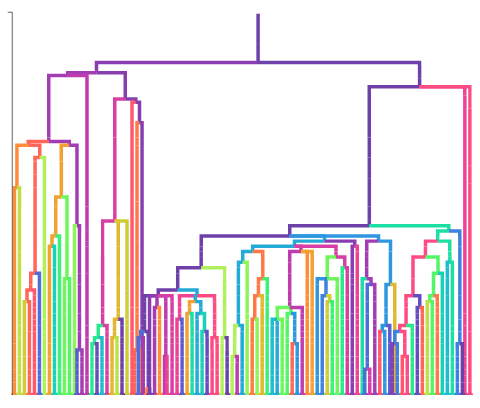
\includegraphics[width=\textwidth, height=0.13\textheight]{img/reference}
    \caption{%
      reference tree}
    \label{fig:plain-perfect-and-reconstruction-phylogenies:reference}
  \end{subfigure}
  \begin{subfigure}[b]{\linewidth}
    \centering
    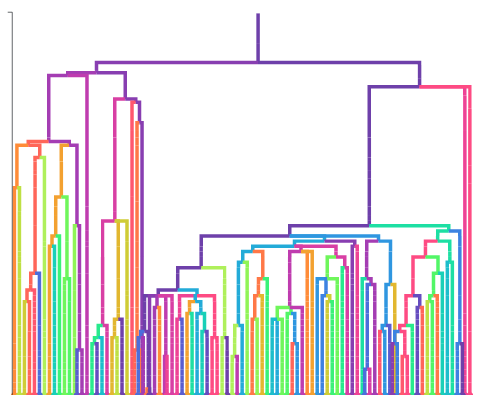
\includegraphics[width=\textwidth, height=0.13\textheight]{img/plain_resolution_100}
    \caption{%
      1\% resolution}
    \label{fig:plain-perfect-and-reconstruction-phylogenies:resolution_100}
  \end{subfigure}
  \begin{subfigure}[b]{\linewidth}
    \centering
    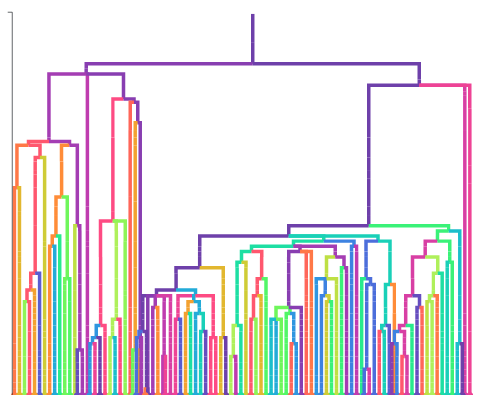
\includegraphics[width=\textwidth, height=0.13\textheight]{img/plain_resolution_30}
    \caption{%
      3\% resolution}
    \label{fig:plain-perfect-and-reconstruction-phylogenies:resolution_30}
  \end{subfigure}
  \begin{subfigure}[b]{\linewidth}
    \centering
    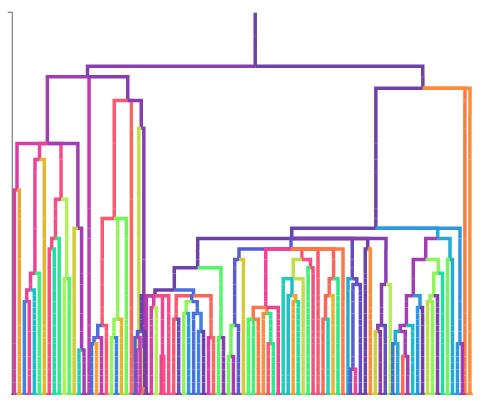
\includegraphics[width=\textwidth, height=0.13\textheight]{img/plain_resolution_10}
    \caption{%
      10\% resolution}
    \label{fig:plain-perfect-and-reconstruction-phylogenies:resolution_10}
  \end{subfigure}
  % \begin{noindent}
  \begin{subfigure}[b]{\linewidth}
    \centering
    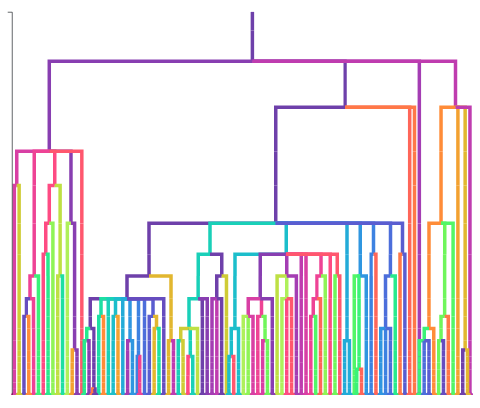
\includegraphics[width=\textwidth, height=0.13\textheight]{img/plain_resolution_3} \caption{%
      33\% resolution}
    \label{fig:plain-perfect-and-reconstruction-phylogenies:resolution_3}
  \end{subfigure}
  % \end{noindent}
  \caption{%
  \textbf{Comparison of phylogeny reconstructions across different hereditary stratigraphy resolutions in the plain evolutionary regime.}
    To maintain visual legibility, these trees contain the same sub-sample of 100 leaf nodes out of the 32,768 in the full trees.
    Sub-figures are arranged from top to bottom in coarsening order of reconstruction resolution.
    Taxon and branch color coding is consistent across subpanels.
    Visit \url{mmore500.com/hstrat-evolutionary-inference/} for mouseover-based highlighting of corresponding clades between reconstructions and reference.
  }
  \label{fig:plain-perfect-and-reconstruction-phylogenies}
\end{figure}


To assess the efficacy of the new agglomerative tree-building approach, we calculated all reconstructed trees' quartet distance to their respective reference.
Quartet distance ranges from 0 (between identical trees) to 0.75 (between random trees), providing in this case a measure of reconstruction error.
As expected, this measure of reconstruction error varied significantly with resolution for trees across all evolutionary regimes (Kruskal-Wallis tests; all $p < 10^{-20}$; Supplementary Table \ref{tab:reconstruction-error-comparisons-between-resolutions}).
Reconstruction error also varied significantly with evolutionary regime for each reconstruction resolution level (Kruskal-Wallis tests; all $p < 10^{-8}$; Supplementary Table \ref{tab:reconstruction-error-comparisons-between-regimes}).

For 3\% and 1\% resolutions, mean reconstruction error was less than 0.01 in all cases and at 10\% resolution mean reconstruction error was less than 0.05 in all cases.
At 33\% resolution, mean reconstruction error was less than 0.12 in all cases.
The largest reconstruction errors observed at 1\%, 3\%, 10\%, and 33\% resolutions were, respectively, 0.051 (weak selection regime), 0.093 (weak 4 niche ecology regime), 0.14 (plain evolutionary regime), and 0.45 (plain evolutionary regime).
Supplementary Table \ref{tab:tree-reconstruction-quality-quartet-summary-statistics} reports mean, median, standard deviation, and maxima for reconstruction error across surveyed evolutionary conditions.

To generate reconstructed trees in experiments, we simulated the inheritance of hereditary stratigraphic annotations along a reference phylogeny to yield the set of annotations that would be attached to extant population members at the end of a run, then used our agglomerative tree building technique to infer.
Thus, each reconstruction replicate has a directly-corresponding reference tree from a perfect-tree treatment replicate.
Figure \ref{fig:plain-perfect-and-reconstruction-phylogenies} shows a reference tree and corresponding reconstructions performed using 1\%, 3\%, 10\%, and 33\% resolution hereditary stratigraph annotations.

\subsection{Phylometrics}

A wide range of metrics exists for quantifying the topology of a phylogeny.
Tucker et.
al showed that these metrics can be classified into the following three dimensions: richness, divergence, and regularity \citep{tuckerGuidePhylogeneticMetrics2017}.
Richness metrics quantify the amount of phylogenetic diversity/evolutionary history represented by a phylogeny.
Divergence metrics quantify how different the units of the phylogeny are from each other.
Regularity metrics quantify the variance of other properties (i.e. how consistent they are across the phylogeny).
Here, we focus on four metrics spread across these categories:

\textbf{Number of Internal Nodes:} This measurement simply counts the number of non-extant taxa in the phylogeny (i.e. the number of non-leaf nodes).
Because the reconstructed trees do not contain any internal nodes not associated with a branching point (i.e. unifurcations), we strip such nodes out of the reference trees as well.
It is a metric of phylogenetic richness and is closely related to Faith's classic phylogenetic diversity metric \citep{faithConservationEvaluationPhylogenetic1992}, the primary differences being that the number of internal nodes is unaffected by branch lengths and the number of leaf nodes.
Consequently, we would expect it to be increased by the presence of ecology or spatial structure, as both these factors increase diversity.

\textbf{Colless-like Index:}
The original Colless Index \citep{collessReviewPhylogeneticsTheory1982}, also often referred to as $I_c$ \citep{shaoTreeBalance1990}, is a measure of tree imbalance (i.e. it gets higher as the tree gets less balanced).
In the context of Tucker et.
al's framework, it is a regularity metric.
However, the traditional Colless Index only works for strictly bifurcating trees.
As our trees have multifurcations, we instead use the Colless-like Index, which is an extension of the Colless Index to multifurcating trees \citep{mirSoundCollesslikeBalance2018}.
Tree imbalance is thought to be associated with varying ecological pressures \citep{chamberlainPhylogeneticTreeShape2014, burressEcologicalOpportunityAlters} and has also been observed to increase in the presence of spatial structure \citep{scottInferringTumorProliferative2020}.

\textbf{Mean Pairwise Distance:}
This metric is calculated by computing the shortest distance between all pairs of leaf nodes and taking the mean of these values \citep{webbExploringPhylogeneticStructure2000}.
Note that these distances are measured in terms of the number of nodes in between the pair, not in terms of branch lengths.
Mean pairwise distance is a metric of evolutionary divergence \citep{tuckerGuidePhylogeneticMetrics2017}.
Mean pairwise distance should be increased by scenarios that promote the long-term maintenance of distinct phylogenetic branches, such as ecology.
Conversely, factors that act to reduce diversity should also reduce mean pairwise distance.

\textbf{Mean Evolutionary Distinctiveness:}
Evolutionary distinctiveness is a metric that can be calculated for individual taxa to quantify how evolutionarily different that taxon is from all other taxa in the phylogeny \citep{isaacMammalsEDGEConservation2007}.
To get mean evolutionary distinctiveness, we average this value across all extant taxa in the tree.
Like mean pairwise distance, mean evolutionary distinctiveness is a metric of evolutionary divergence.
However, it is known to capture substantially different information than mean pairwise distance \citep{tuckerGuidePhylogeneticMetrics2017}.
Unlike our other metrics, evolutionary distinctiveness is heavily influenced by branch length.
We generally expect mean evolutionary distinctiveness to be increased by similar factors to mean pairwise distance.

\subsection{Software and Data Availability}

Software, configuration files, and executable notebooks for this work are available at \url{https://github.com/anony4review/hstrat-evolutionary-inference}.
% \begin{noindent}
Data and supplemental materials are available via the Open Science Framework \url{https://osf.io/vtxwd/?view_only=4dd2cd7ee24b450d96358f891a41414f} \citep{foster2017open}.
% \end{noindent}

All hereditary stratigraph annotation, reference phylogeny generation, and phylogenetic reconstruction tools used in this work are published in the \texttt{hstrat} Python package \citep{moreno2022hstrat}.
This project can be visited at \url{https://github.com/mmore500/hstrat}.

This project uses data formats and tools associated with the ALife Data Standards project \citep{lalejini2019data} and benefited from many pieces of open-source scientific software \citep{ofria2020empirical,sand2014tqdist,2020SciPy-NMeth,harris2020array,reback2020pandas,mckinney-proc-scipy-2010,sukumaran2010dendropy,cock2009biopython}.
